\documentclass[11pt]{article}
\usepackage[margin=1in]{geometry}
\usepackage{amsmath,amssymb,graphicx,microtype,booktabs}
\usepackage[font=small,skip=3pt]{caption}
\usepackage[hidelinks]{hyperref}
\usepackage{enumitem}
\setlist{nosep,leftmargin=1.2em}
\setlength{\parindent}{0pt}
\setlength{\parskip}{2.5pt plus 1pt minus 1pt}
\setlength{\textfloatsep}{5pt plus 2pt minus 2pt}
\setlength{\intextsep}{7pt plus 2pt minus 2pt}
\title{\vspace{-1.6em}\textbf{Proof Space Has More Than One Geometry}\vspace{-0.5em}}
\author{J. R. Landers\\[-1pt]\small Connecting three Lean experiments to the literature}
\date{\vspace{-1.2em}}

\begin{document}
\maketitle
\vspace{-1.6em}

The phrase \emph{proof space} invites a picture: theorems and proofs occupy positions, nearby
objects resemble one another, and a successful prover moves through the resulting landscape.
Several literatures make versions of this picture precise, but they do not describe the same
space.  Proof theory studies transformations of proofs.  Type theory can make identity itself
path-like.  Formal libraries form dependency networks.  Representation learning places symbolic
objects in numerical spaces whose distances support search.

Three experiments on LeanDojo Benchmark 4 approached the last picture from complementary views.
\emph{Textures of Modern Formal Mathematics} separated tactic style from premise-defined subject
on 10,000 recorded proofs \cite{textures}.  \emph{What Statements Know, What Proofs Do} recovered
the distinction in learned embeddings and found a local bridge between the two views
\cite{statements}.  \emph{Nearby Examples, New Proofs} tested that bridge by retrieving examples
for generative proof search and submitting every candidate to Lean \cite{nearby}.  Read together
with earlier and contemporary work, the sequence suggests neither one universal point cloud nor
three unrelated metaphors.  It suggests a \emph{multiplex geometry}: intrinsic, structural, and
learned relations coexist, with explicit maps---and information loss---between them.

\paragraph{Three uses of geometry.}
Let $\mathcal{T}=\{t_1,\ldots,t_n\}$ be $n$ formal theorem statements and let
$\mathcal{P}=\{p_1,\ldots,p_n\}$ contain one recorded proof artifact $p_i$ for each statement
$t_i$.  Here an artifact may be a tactic trace or proof source, not merely the elaborated kernel
term.  Three kinds of structure can be put on these sets.

First, an \emph{intrinsic} geometry comes from the logic.  Girard's proof nets remove inessential
sequential order from linear-logic derivations, while the geometry of interaction interprets
cut elimination as an execution process \cite{girard}.  Homotopy type theory gives a different
literal geometry: an equality proof between terms $a$ and $b$ is a path from $a$ to $b$, and
equalities between equality proofs form higher paths \cite{hott}.  These constructions concern
proof identity, composition, and normalization; their notion of sameness is logically controlled.

That point is decisive for Lean.  Propositions live in the proof-irrelevant sort
\texttt{Prop}: if $u$ and $v$ both prove proposition $A$, Lean treats $u$ and $v$ as equal for
definitional equality \cite{lean4}.  Tactic traces can nevertheless differ in length, vocabulary,
intermediate states, and automation.  Our proof embeddings distinguish these construction
artifacts, not kernel-level evidence modulo proof irrelevance.  They are therefore not an
approximation to a metric that Lean assigns to proofs; Lean assigns no such metric.

More formally, let $\mathcal{F}_i$ be the \emph{artifact fiber}: all tactic scripts that elaborate
to a term of type $t_i$, and let $\varepsilon_i:\mathcal{F}_i\to\{u:u:t_i\}$ be elaboration.
Proof irrelevance collapses the terms in the codomain, while our style features and proof vectors
place geometry on the domain $\mathcal{F}_i$.  Girard's constructions motivate quotienting away
sequential bureaucracy, but our tactic model does not perform that logical quotient; it measures
which bureaucracy recurs.  Homotopy type theory enriches the codomain with paths and higher paths,
whereas one-proof-per-theorem data sample only one point from each empirical fiber.

Second, a \emph{structural} geometry comes from the library.  Let $V$ be the declarations in a
formal corpus and define the dependency matrix $D$ by
\[
 D_{ij}=\begin{cases}
 1,&\text{if the proof of declaration $i$ uses declaration $j$,}\\
 0,&\text{otherwise.}
 \end{cases}
\]
A row of $D$ is a theorem's premise neighborhood; directed paths record transitive dependence.
When one proof step can involve several declarations jointly, a hyperedge---an edge joining any
number of vertices---retains information that an ordinary pairwise edge can lose.  Cross-library
concept alignment already used such formal structure to recover analogous constants across six
proof assistants \cite{alignment}.  At Mathlib scale, Li et al. map 308,129 declarations and
8.4 million dependency edges, showing both modular organization and substantial cross-namespace
coupling \cite{network}.  Barkeshli, Douglas, and Freedman go further: their universal proof and
structural hypergraphs propose a mathematical object in which proofs, definitions, and theories
can be compared globally \cite{structure}.

Third, a \emph{learned} geometry is induced by a representation.  For encoders $f_S$ and $f_P$,
define unit vectors
\[
 x_i=\frac{f_S(t_i)}{\lVert f_S(t_i)\rVert_2},\qquad
 y_i=\frac{f_P(p_i)}{\lVert f_P(p_i)\rVert_2},\qquad
 \lVert z\rVert_2=\left(\sum_r z_r^2\right)^{1/2},
\]
where $\lVert z\rVert_2$ is the Euclidean norm of vector $z$.  The two cosine-similarity kernels
are $K_S(i,j)=x_i\mathbin{\cdot}x_j$ and $K_P(i,j)=y_i\mathbin{\cdot}y_j$, where the dot
denotes the sum of componentwise products.  Cosine distance is $1-K_S(i,j)$ in statement space
and $1-K_P(i,j)$ in proof space.  These distances depend on the corpus, serialization, model, and
training objective.  Unlike intrinsic equivalence, they may change under a harmless renaming or
under replacement of a proof by another proof of the same statement.

The first note's domain formalism is a compression of the structural layer.  If $X^{(d)}$ is its
nonnegative TF--IDF matrix of cited premises and namespaces, then
$X^{(d)}\approx W^{(d)}H^{(d)}$ with $W^{(d)},H^{(d)}\geq0$ expresses each theorem as a mixture of
recurring dependency neighborhoods.  Here $W^{(d)}$ contains theorem-topic weights and $H^{(d)}$
contains topic-feature weights.  This is a low-rank, namespace-coarsened view of rows of $D$, not a
replacement for the full Mathlib graph.  The analogous style factorization compresses tactic
sequences.  Their AMI therefore compares two lossy maps from proof artifacts---one through
incidence structure and one through procedural vocabulary.

\paragraph{Where representation learning enters.}
Continuous representations for theorem proving predate modern Lean models.  Purga\l, Parsert,
and Kaliszyk trained reversible first-order-logic embeddings to preserve syntactic and semantic
properties and tested them on Mizar premise selection \cite{vectors}.  Their central question---
which logical properties should survive compression into a vector?---also exposes the limitation
of our general-purpose text encoder: its geometry is observed after training rather than specified
by a logical objective.

Later systems connect representation directly to formal search.  LeanDojo couples a dense retriever
to a tactic generator, making premises selected from a large Lean library available at each proof
state \cite{leandojo}.  LeanSearch embeds informal queries and formal declarations for semantic
search in Mathlib \cite{leansearch}.  In Coq, Graph2Tac reports that physical locality predicts
relevance and that nearby lemmas often have similar proof structure; online representations improve
proving in unseen developments \cite{graph2tac}.  Samoylov and Vosoughi sharpen the procedural side
for Lean by representing a tactic through the change it induces between the proof state before and
after its application \cite{operators}.  Their operator view supplies a natural refinement of our
surface tactic traces: proofs can be compared by what their steps \emph{do}, not only by which tactic
names occur.

Our unigrams and bigrams record tactic occurrence and order; effect-grounded embeddings record
proof-state transitions.  Replacing the former by the latter would test whether content--procedure
separation survives a representation closer to proof-theoretic dynamics.

\begin{figure}[t]
  \centering
  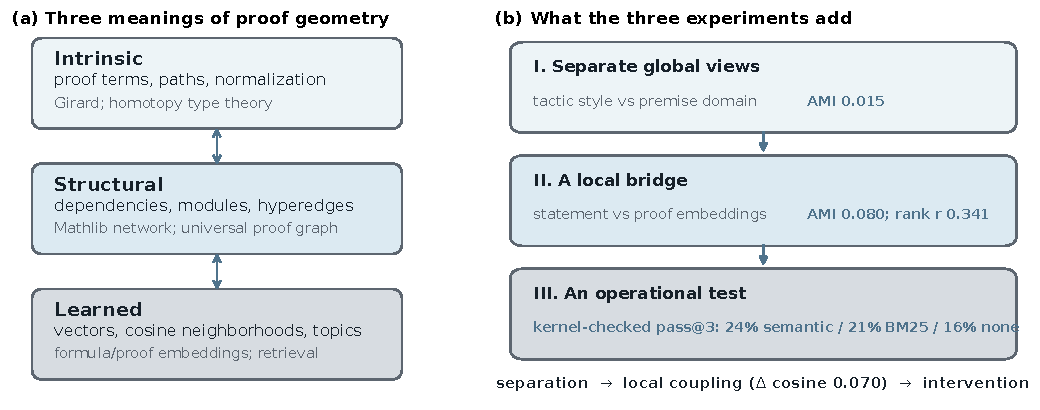
\includegraphics[width=\textwidth]{proof_geometry_synthesis.pdf}
  \caption{A synthesis rather than an identification.  (a) Intrinsic, structural, and learned
  geometries place different relations on formal mathematics; maps between layers discard some
  structure.  (b) The three-note sequence measures separation, a local cross-view bridge, and an
  operational consequence.  AMI is adjusted mutual information; $r_s$ is Spearman rank
  correlation; pass@3 is the fraction solved within three candidates.  Values are read directly
  from the archived experimental artifacts.}
  \label{fig:synthesis}
\end{figure}

Chen and Li make the geometry/search connection theoretical.  Starting from a theorem graph with
semantic edges, they use diffusion similarity and contrastive Euclidean embeddings to analyze
self-play theorem proving \cite{selfplay}.  Our measurements qualify the single-graph assumption.
There is evidence for semantic edges, but statement and proof relations are not interchangeable;
a theorem graph should specify which layer generates an edge and how information crosses layers.

\paragraph{What the first two notes add.}
The first note constructed two proof-by-feature matrices: tactic-head unigrams and bigrams for
procedure, and cited premises and namespaces for subject.  Independent TF--IDF weighting and
nonnegative matrix factorization produced eight style topics and ten domain topics.  Their
adjusted mutual information was $0.015$, where adjusted mutual information (AMI) is cluster-label
agreement corrected so that its expectation under random fixed-size partitions is approximately
zero and identical partitions score one.  Coarse Mathlib module labels agreed much more with domain
topics (AMI $0.241$) than style topics (AMI $0.025$) \cite{textures}.  In structural terms, the
domain vector is a weighted local signature of a row of $D$; the style vector describes a path
through tactics.  The low alignment is thus evidence that dependency neighborhood and procedure
are distinct coordinates, not evidence that either lacks structure.

The second note replaced designed features with 1,024-dimensional embeddings of statements,
proofs, and their concatenation.  Global statement and proof clusterings still differed
(AMI $0.080$), while the joint view resembled statements more than proofs \cite{statements}.
The companion neighborhood test then supplied the positive half of the result.  Across 500,000
sampled theorem pairs, $K_S(i,j)$ and $K_P(i,j)$ had Spearman rank correlation $r_s=0.341$, where
$r_s$ is the ordinary Pearson correlation of the two variables' ranks.  For each theorem, the
top-ten statement and proof neighbor sets overlapped by $0.134$ on average, versus random
expectation $0.001$.  Proof cosine among top-ten statement neighbors was $0.6727$, compared with
$0.6030$ for random neighbors matched by source-file and module relationship, a difference of
$0.0696$ with theorem-bootstrap 95\% interval $[0.0687,0.0705]$.

Low global partition agreement together with positive local association matches Graph2Tac's
locality observation while separating two axes that its proving objective combines.
It also differs from concept alignment: Gauthier and Kaliszyk search for correspondences between
libraries, whereas our paired views concern one theorem and one recorded proof inside one library.
The result says that nearby statements make nearby proof artifacts more likely, not that a
statement determines a canonical proof.

\paragraph{The closest direct comparison.}
Mendoza-Smith's study of choice in neural proof embeddings is the nearest precedent in both object
and method \cite{choice}.  It partitions 471,260 Mathlib declarations by transitive dependence on
\texttt{Classical.choice}, trains a self-supervised encoder on constructive proofs, and studies
42,355 traced proofs.  Anomaly score, reconstruction loss, and density-superlevel containment all
separate shallow classical proofs from the constructive distribution: anomaly discrimination has
area under the receiver-operating-characteristic curve $0.847$ at dependency distance two, then
fades to indistinguishability by distance nine or greater.  A mixture model
\[
 Q_d=(1-\lambda_d)P+\lambda_d R,
\]
describes the trend, where $d$ is dependency distance from choice, $P$ is the constructive proof
distribution, $R$ is a residual distribution, and $0\leq\lambda_d\leq1$ is the residual weight at
distance $d$.  The learned anomaly score also predicts prover behavior beyond proof length.

The two programs are complementary.  The choice study starts with a kernel-traceable foundational
label and asks whether that axis leaves a signature.  Our notes start without such a label and ask
which content and procedural axes emerge, whether they couple locally, and whether retrieval helps.
Its sharpest separation occurs at a dependency boundary; ours is more diffuse but extends through
an intervention.  Both connect geometric distance to prover outcomes.

\paragraph{From map to mechanism.}
The third note turns locality into a treatment.  On 100 held-out targets, prompts use no examples,
random examples, BM25 lexical retrieval, or semantic statement retrieval.  BM25 favors rare query
tokens while correcting for document length and repetition.  Each condition receives three
candidates, all checked by Lean in their original source context.  Pass@3 is $16\%$ without retrieval,
$14\%$ with random examples, $21\%$ with BM25, and $24\%$ with semantic retrieval
\cite{nearby}.  Semantic retrieval beats random retrieval by ten paired percentage points
(95\% bootstrap interval $[3,18]$), but its three-point advantage over BM25 is not resolved
($[-3,9]$).  This is operational evidence for useful neighborhoods, not evidence that cosine
similarity has isolated a uniquely mathematical notion of relevance.  Lexical and semantic
routes can reach many of the same solvable targets through different examples.

\paragraph{A multiplex model.}
The synthesis can be stated without forcing the layers into one metric.  Let
\[
 \mathcal{M}=(V_S\sqcup V_P,\,E_S,E_P,E_{SP},D),
\]
where $V_S=\{t_i\}$ and $V_P=\{p_i\}$ are disjoint statement and proof vertices; $E_S$ and $E_P$
are weighted edges derived from $K_S$ and $K_P$; $E_{SP}=\{(t_i,p_i):1\leq i\leq n\}$ pairs each
statement with its recorded proof; and $D$ records library dependencies.  The symbol $\sqcup$
means disjoint union.  Intrinsic proof transformations can be added as typed edges on elaborated
terms, but should not be identified with empirical similarity.

For computation, let $W_S$ and $W_P$ be nonnegative weighted adjacency matrices obtained by
retaining selected entries of $K_S$ and $K_P$.  A two-layer adjacency is
\[
 A_\eta=\begin{pmatrix}W_S&\eta I_n\\ \eta I_n&W_P\end{pmatrix},\qquad \eta\geq0,
\]
where $I_n$ is the $n\times n$ identity matrix and $\eta$ weights statement--proof pairing edges.
At $\eta=0$ the learned graphs are separate; increasing $\eta$ lets a walk cross between paired
views.  Chen and Li's diffusion similarity can operate on $A_\eta$ rather than on one
undifferentiated theorem graph.  Low global AMI but positive local correlation predicts an
intermediate regime: enough coupling for retrieval, not enough to identify the layers.  Adding
edges from $D$ supplies the structural third layer proposed by the Mathlib-network and
universal-hypergraph programs.

This model turns the connections into tests.  Dependency-aware encoders ask how much of $E_S$ and
$E_P$ is predicted by $D$; effect-grounded encoders replace surface proof edges by proof-state
transitions.  Multiple proofs replace one pairing edge by a fiber---all observed proofs above one
statement---separating within-theorem from across-theorem variation.  Perturbations can test
invariance to renaming, refactoring, and equivalent statements.  Retrieval can then draw examples
from statement, proof, dependency, or fused neighborhoods and let the kernel decide which helps.

The literature supplies more than precedent: proof theory removes administrative syntax, type
theory structures identity, library networks expose dependence, representation learning makes
proximity useful, and kernel checking tests utility.  The experiments occupy the interfaces.  Their
result is not a reduction of proof to vectors, but distinguishable content, procedural, and
dependency geometries whose partial alignment is measurable and actionable.

\begin{thebibliography}{99}\scriptsize
\setlength{\itemsep}{0pt}
\bibitem{textures} J. R. Landers. ``Textures of Modern Formal Mathematics.'' Remarks on LeanDojo Benchmark 4, 2026.
\bibitem{statements} J. R. Landers. ``What Statements Know, What Proofs Do.'' Semantic views of LeanDojo Benchmark 4, 2026.
\bibitem{nearby} J. R. Landers. ``Nearby Examples, New Proofs.'' Retrieval-guided generation in LeanDojo Benchmark 4, 2026.
\bibitem{girard} J.-Y. Girard. ``Linear Logic.'' \emph{Theoretical Computer Science} 50, pp. 1--102, 1987; ``Geometry of Interaction I: Interpretation of System F.'' In \emph{Logic Colloquium '88}, pp. 221--260, 1989.
\bibitem{hott} The Univalent Foundations Program. \emph{Homotopy Type Theory: Univalent Foundations of Mathematics}. Institute for Advanced Study, 2013.
\bibitem{lean4} L. de Moura and S. Ullrich. ``The Lean 4 Theorem Prover and Programming Language.'' CADE 28, pp. 625--635, 2021.
\bibitem{alignment} T. Gauthier and C. Kaliszyk. ``Aligning Concepts across Proof Assistant Libraries.'' \emph{Journal of Symbolic Computation} 90, pp. 89--123, 2019.
\bibitem{vectors} S. Purga\l, J. Parsert, and C. Kaliszyk. ``A Study of Continuous Vector Representations for Theorem Proving.'' \emph{Journal of Logic and Computation} 31(8), pp. 2057--2083, 2021.
\bibitem{leandojo} K. Yang et al. ``LeanDojo: Theorem Proving with Retrieval-Augmented Language Models.'' NeurIPS Datasets and Benchmarks, 2023.
\bibitem{leansearch} G. Gao et al. ``A Semantic Search Engine for Mathlib4.'' Findings of EMNLP, pp. 8001--8013, 2024.
\bibitem{graph2tac} L. Blaauwbroek et al. ``Graph2Tac: Online Representation Learning of Formal Math Concepts.'' ICML, PMLR 235, pp. 4046--4076, 2024.
\bibitem{operators} E. Samoylov and S. Vosoughi. ``Modeling Tactics as Operators: Effect-Grounded Representations for Lean Theorem Proving.'' MathNLP, pp. 168--175, 2025.
\bibitem{network} X. Li, N. Peng, S. Severini, and P. Shafto. ``The Network Structure of Mathlib.'' arXiv:2604.24797, 2026.
\bibitem{structure} M. Barkeshli, M. R. Douglas, and M. H. Freedman. ``Artificial Intelligence and the Structure of Mathematics.'' arXiv:2604.06107, 2026.
\bibitem{selfplay} T. Chen and Z. Li. ``A Theoretical Framework for Self-Play Theorem Proving Algorithms.'' arXiv:2606.01861, 2026.
\bibitem{choice} R. Mendoza-Smith. ``Geometric Measurements of the Axiom of Choice in Neural Proof Embeddings.'' arXiv:2606.28572, 2026.
\end{thebibliography}

\end{document}
